\chapter{Design Considerations}
\label{cha:designConsiderations}
	
	%----------
	\section{Fundamental Approach}
		\textit{STORM} is a framework to generate code for an object-relational mapper on
		basis of templates. There are a few question which need to be answered before starting
		a design for the framework. These questions are:
		
		\begin{enumerate}
			\item	What needs to be parameterised?
			\item How can parameters be defined?
			\item How can parameters be passed to templates?
		\end{enumerate}
		
		\subsection{What needs to be parameterised?}
			Obviously, for an object-relational mapper the most important thing to parameterise
			is the mapping. This means, the database structure, the structure of the in-memory objects
			and the mapping between them must be defined. For example, one needs to be able to define
			that an in-memory object of a class \verb~Person~ maps to a database table called \verb~Persons~.
			Not only the structure must be configurable but also primary keys,
			foreign keys and relations between tables.
		
		\subsection{How can parameters be defined?}
			After we know \emph{what} needs to be parameterised, the question is \emph{how}. At the beginning
			of this thesis, three different fundamental approaches were analysed and tested.
			
			The first approach is XML Schema: There are two XML Schema files and one plain XML file.
			One XML Schema file is to define the in-memory object structure, the other one is to define
			the database structure and the XML file is used to describe the mapping between the two.
			The problem of this approach is its complexity and unmanageability.
			
			Another approach was an extended C\# compiler. This compiler would work with custom defined
			keywords. This keywords could be used to define the structures and mapping.
			
			The third approach to describe the mapping is to write an abstract class
			with custom attributes. A code snippet of such a class is shown in Listing
			\ref{lst:abstractClassAdr}. After compiling this has been compiled, the custom
			attributes can be read using reflection from the resulting dll. With these attributes,
			all relevant information can be retrieved.
			
					\begin{lstlisting}[float=htb,language={[Sharp]C},caption=Abstract class with custom attributes,label=lst:abstractClassAdr]
	[Table("Addresses", true),
	VersionField("chTimeStamp"),
	GenerateCode]
	public abstract class Address : DomainObject
	{
		[Factory]
		public abstract class AddressFactory
		{
			public abstract Address createAddress(
			[ParameterDef("City")] string city,
			[ParameterDef("Street")] string street,
		}

		[Column("AddressID"),
		PrimaryKey]
		public abstract int AddressId {get;}

		[ToMany(typeof(OrderDetail), "OrderId")]
		public abstract IList OrderDetails {get;}

		[Column("PersonID"),
		ToOne(typeof(Person), "PersonId")]
		public abstract Person PersonRel {get; set;}

		[Column("City")]
		public abstract string City {get; set;}

		[Column("Street")]
		public abstract string Street {get; set;}
	}
}
			\end{lstlisting}
			
			The main advantage of this is that a programmer can define everything in a single file (single-source approach)
			rather than multiple files. This means, not only the mapping code could be generated automatically, but also
			the corresponding database tables. Furthermore it is a natural way for programmers because
			they are used to write classes.
			
			One could say that a drawback of attributes is that they cannot be changed at runtime.
			This is true but also, it is not required. Every information given in this 
			abstract class is static within the scope of an application. 
			
			From our point of view, this approach is the most feasible. 
			
		\subsection{How can parameters be passed to templates?}
			Once we know how to parameterise everything we need a way to let the 
			template know all these parameters. The first thing which is given is that
			custom attributes in C\# are bound to the class in in which they are defined.
			Therefore, attributes must be read by using reflection. First, we could
			generate code which makes use of reflection or second, we use reflection
			in the template itself an generate code containing no reflection but the 
			concrete code resulting from the custom attributes. The latter case is more
			according to the idea of generative programming. If we used reflection
			in the generated code the application's performance would be poorer. What is more,
			it would not make much sense because we would not need to write any templates
			at all.
								
	%----------
	\section{Object Dependencies}
		Whenever code is generated, it is important to design the application carefully.
		An important consideration must be object dependencies. This is, an abstract class or any
		class written in the client code
		may never depend on a generated class nor may a generated class depend on
		another generated class. If such a dependency existed, it would result in a dependency
		cycle which cannot be resolved. Consider an abstract class \verb~Person~ which results
		in the concrete implementation class \verb~PersonImpl~. Further, consider a client 
		which wants to set the property \textit{Name} for a \verb~Person~ and uses the concrete
		implementation \verb~PersonImpl~ for this (see Figure \ref{fig:DesignObjectDependency}). This
		would have the effect that the client class could not be compiled before the concrete
		implementation is generated. But to generate the concrete implementation, the client code
		needs to be compiled (because the resulting dll is needed). This could be avoided by putting
		the client code in a separate project. But at the latest when you have dependencies between
		abstract classes and concrete implementation classes this cannot be avoided.
		
		Therefore a mechanism is needed that the client code just need to reference the 
		abstract class but still can set the property in the concrete implementation object.
		For this we use a \textit{Factory Method} which provides us with a concrete implementation without
		the need of referencing it directly. How exactly the \textit{Factory Method} was used is explained
		in \ref{sec:Factory}.
		
		\begin{figure}[htb]
			\begin{center}
				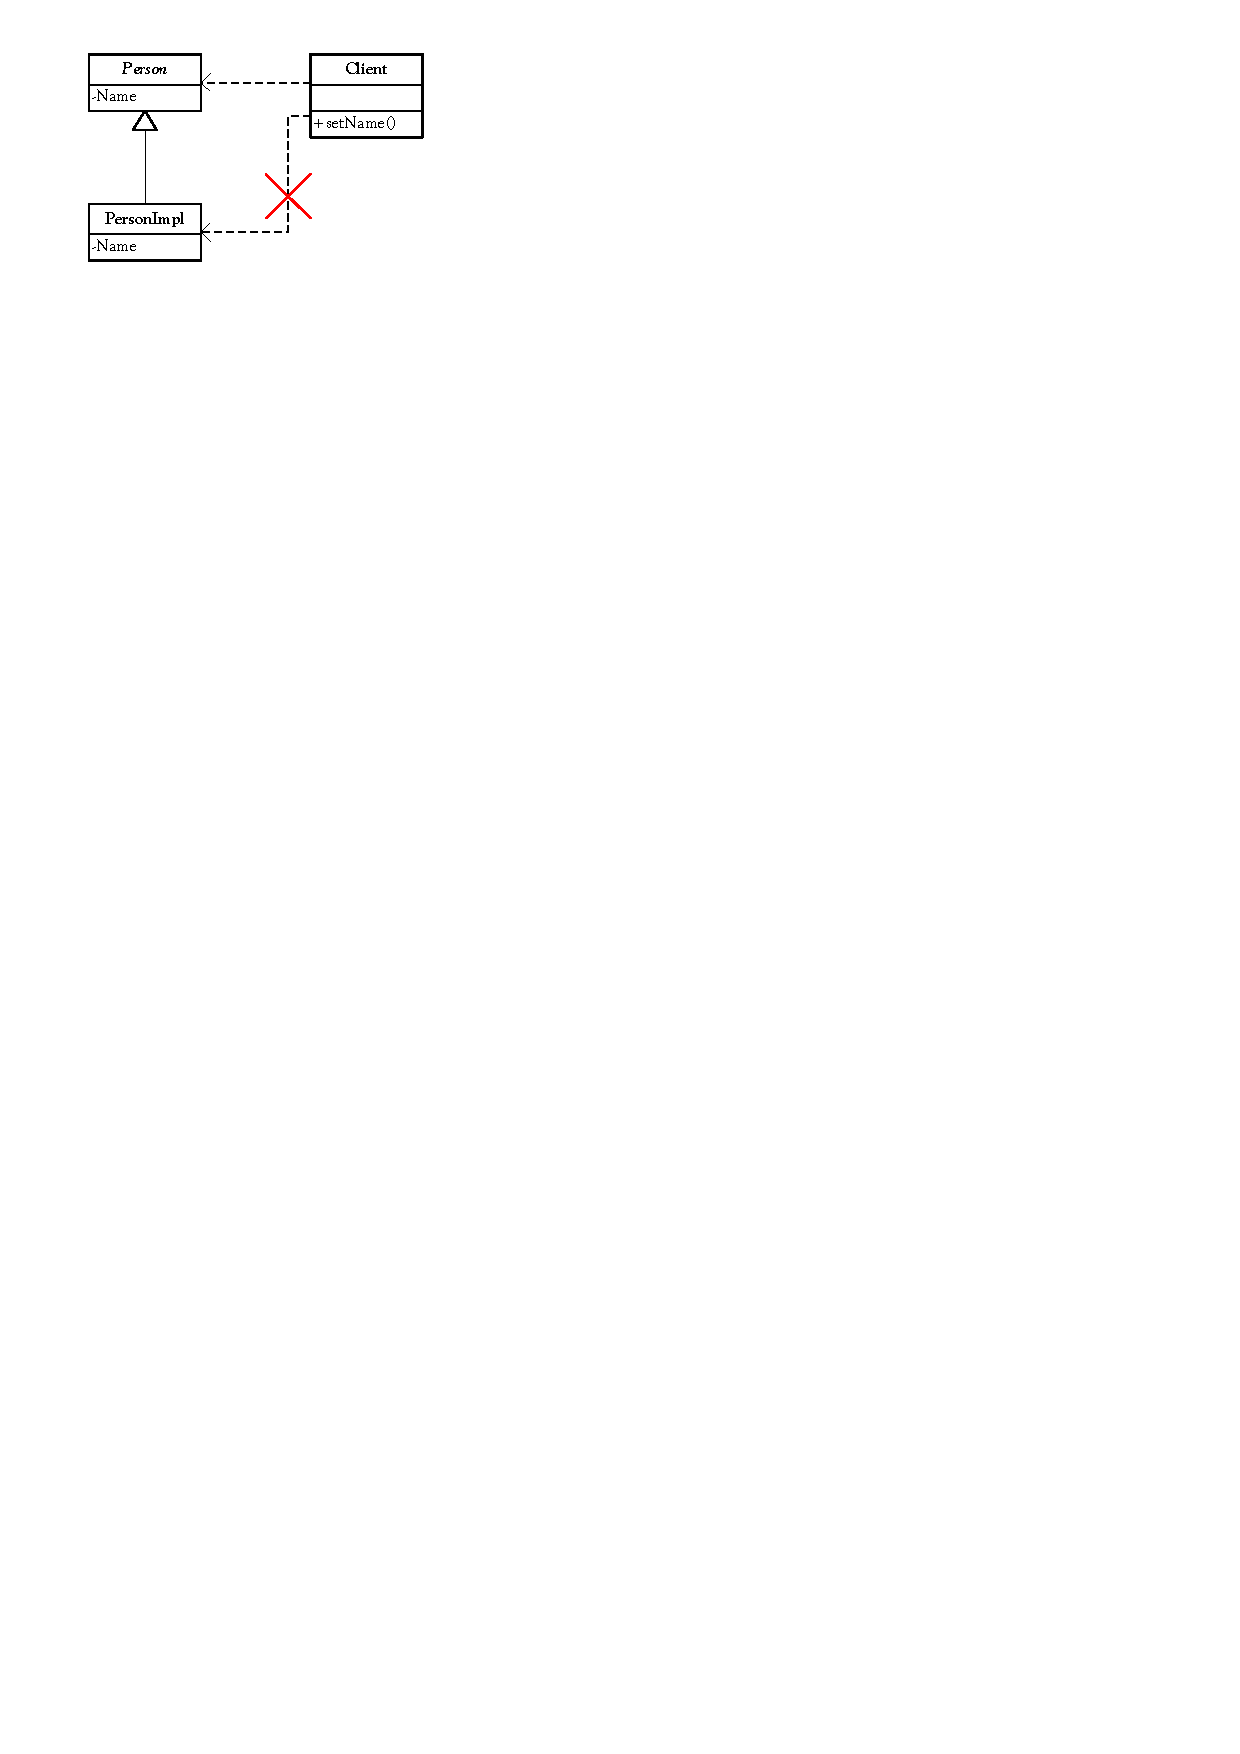
\includegraphics{./files/inc/figures/DesignObjectDependency}
				\caption{\label{fig:DesignObjectDependency} Dependencies between classes}
			\end{center}
		\end{figure}

	%----------
	\section{Object Lifetime}
	\label{sec:objectLifetime}
		An object which has been transferred from the database can be kept for further use in
		an \textit{Identity Map} (see \ref{subsec:identityMap}). The question is, how long this object resides in this
		map. An \textit{Identity Map} is stored in a \textit{Unit of Work} (see \ref{subsec:unitOfWork}) and therefore, if the
		\textit{Unit of Work} object is destroyed, the \textit{Identity Map} and all objects
		stored in it will be destroyed too. This is indicated in Figure \ref{fig:designUoW_IdentityMap}.
		This brings up the question how long a \textit{Unit of Work} object should exists. There are
		two answers for that:
		\begin{itemize}
			\item The objects lifetime is as long as a user session exists. This is, a \textit{Unit of Work}
						object is created on a per thread basis. A new thread is started on each new session.
			\item The object is on a per transaction basis. This is, a new \textit{Unit of Work} object is 
						created on every commit.
		\end{itemize}
		These two methods represent completely different concepts. The first implies that it is possible 
		for an object to reside in an \textit{Identity Map} for a long time. On the one hand, this increases the
		risk of consistency errors but on the other hand, it follows more the idea of an \textit{Optimistic
		Offline Lock} (see \ref{subsec:optimisticOfflineLock}) architecture. This means that
		consistency errors will rarely occur.
		Additionally, we avoid consistency errors by using a lazy load
		system which checks if the object in question is up to date (see \ref{subsec:LazyLoad}).
		
		The second method is more adequate for a system with many users who are likely to
		edit the same object simultaneously. In such
		systems, consistency errors are likely to occur. Whenever this is the case, it makes not
		much sense to store objects in an \textit{Identity Map} for a long time to just remove
		them upon the next update.
		
		We assume that the first case is more appropriate in most cases and use therefore a per
		session based \textit{Unit of Work}.
		
		\begin{figure}[htb]
			\begin{center}
				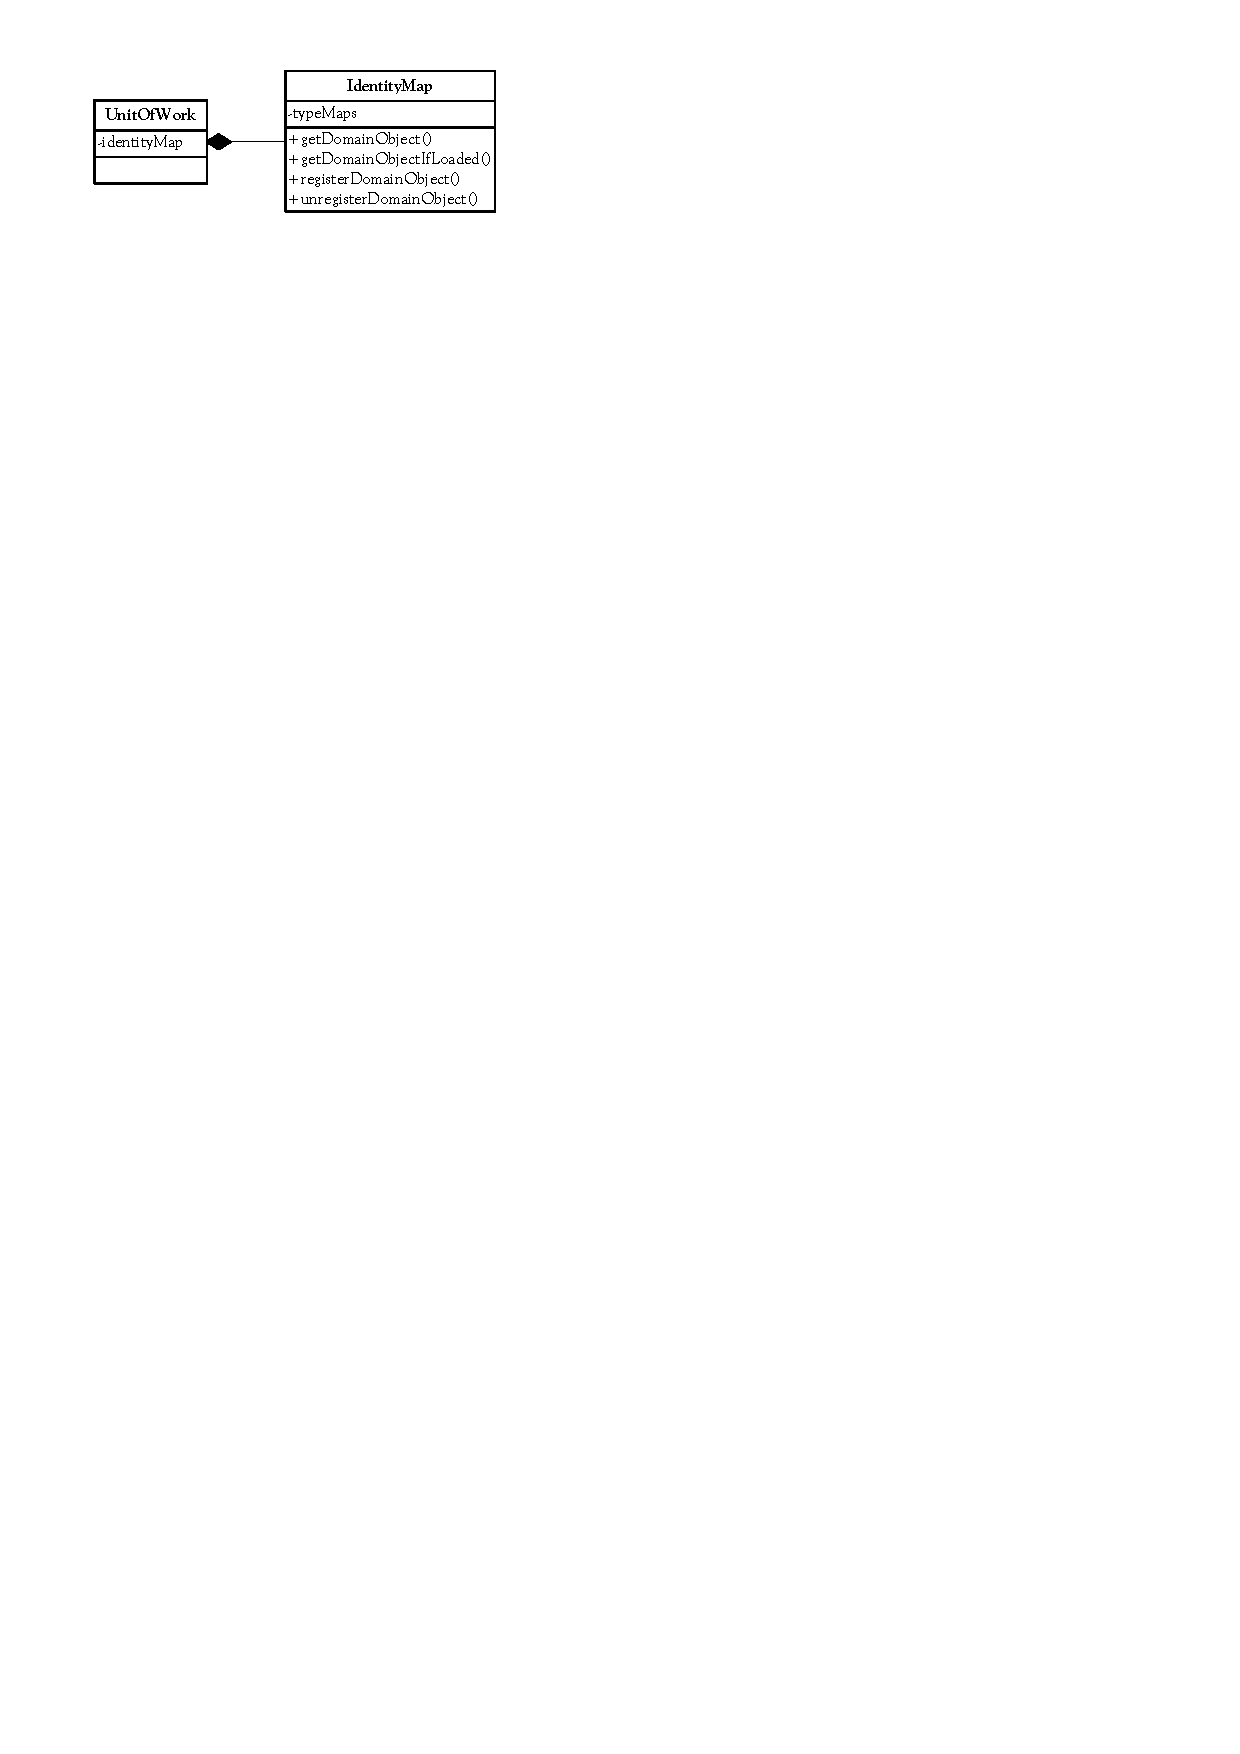
\includegraphics{./files/inc/figures/designUoW_IdentityMap}
				\caption{\label{fig:designUoW_IdentityMap} Relation between \textit{Unit of Work} and an \textit{Identity Map}}
			\end{center}
		\end{figure}
		
	%----------
	\section{Locking Mechanisms}
	\label{sec:lockingMechanisms}
		Depending on the application, different database locking mechanisms are appropriate. There are two
		main ways how database locking can be implemented:
		
		\begin{itemize}
			\item	The whole database is locked during a transaction. 
			\item Only certain records of the database are locked during a transaction.
		\end{itemize}
		
		The first method its easier to implement and adequate for many applications. It locks the
		whole database within a business transaction. The disadvantage of this is that whenever several
		people access the same data within a business transaction, only one of them can commit without 
		a conflict. For all others, the transaction will fail.
		
		The second method solves this problem by using more sophisticated locks. Several strategies
		can be used:
		
		\begin{description}
			\item[exclusive write lock] A business transaction acquires a lock in order to edit session data. Reading 
																	these data is still possible.
			\item[exclusive read lock]	A business transaction is required to acquire a lock simply to load the record.
			\item[read/write lock]			A record cannot be write-locked if any other business transaction owns a
																	read lock on it and vice versa. Concurrent read-locks are acceptable.
		\end{description} 
		
		For this thesis, we use the first method which locks the whole database. The reason is that
		we do not have a concrete application for which a more complicated locking mechanism would
		be needed. But Generally, it is important to choose the right locking strategy.

	%----------
	\section{Mapping Types}
	\label{sec:mappingTypes}
		
		Not all possible mapping types are supported by \textit{STORM}. This section 
		describes the supported types. That is, which elements of the object oriented 
		code can be mapped to which database elements. The custom attributes which define
		the mapping is named for each type.
		A detailed description of the attributes can be found in section \ref{sec:attributes}.
		
		\begin{description}
			\item[Class]                     A class is always mapped to one table. Even though, it would be possible to map 
			                                 more than one class to the same table. 
			                                 
			                                 The \hyperlink{TableAttribute}{Table} attribute is mandatory for each class.
			\item[Member variable]           A member variable of a class is mapped to a column within 
			                                 the corresponding table.
			                                 
			                                 The \hyperlink{ColumnAttribute}{Column} attribute sets the name of the 
			                                 column.
			\item[One to one relation]       A relation from one table to exactly one entry of another table. Table 
			                                 $A$ contains the primary key or a unique key of an entry in table $B$.
			                                 In the source code, this mapping is done by referencing object $A$ to object $B$.
			                                 
			                                 \hyperlink{ToOneAttribute}{ToOne} is the attribute defining this relation.
			\item[One to many relation]      A relation from one table to several entries of another table. 
			                                 A database handles this relation by placing a foreign key in each entry
			                                 in table $B$. With this foreign key, entries in table $B$ know that they belong
			                                 to table $A$.

			                                 In the source code, object $A$ has an array list which contains all related 
			                                 objects $B$. \textit{STORM} needs a back reference (to-one relation) in class 
			                                 $B$ for each to-many relation in class $A$.
			                                 
			                                 \hyperlink{ToManyAttribute}{ToMany} is the attribute defining this relation.
			\item[Many to many relation]     To realise such a relation on the database, an 
				                               linking table is needed to store the relations between entries.

				                               In the code it is possible to manage many-to-many relations 
				                               with array lists without the need of an extra object between them.
				
				                               We do not support this special case. To make a many-to-many relation 
				                               it would be necessary to make an extra object which maps to the linking table.
				                               
			\item[Enumeration/Lookup tables] Enumerations are not needed and often not supported by 
				                               databases. If you are thinking about using an enum you should consider to save 
				                               the values in a lookup table. Enumerations are not supported by \textit{STORM}.
		\end{description}
		
		